\documentclass[12pt,letterpaper]{article}

\usepackage[margin=1in]{geometry}
\usepackage{times}
\usepackage{amsmath}
\usepackage{amssymb}
\usepackage{graphicx}
\usepackage{booktabs}
\usepackage{hyperref}
\usepackage{enumitem}
\usepackage{setspace}
\usepackage{caption}
\usepackage{array}

\hypersetup{colorlinks=true, linkcolor=blue, urlcolor=blue, citecolor=blue}

\setlength{\parskip}{5pt}
\setlength{\parindent}{0pt}

\title{\textbf{Fault-Tolerant Quadrotor Control via\\PID-Guided Reinforcement Learning}}
\author{Swarup Patil (U20220085)\\[4pt]\small Reinforcement Learning Course Project}
\date{May 2026}

\begin{document}
\maketitle
\thispagestyle{empty}

% ================================================================
\section*{1. Problem Statement}
% ================================================================

Quadrotors are widely used in applications ranging from infrastructure inspection to search and rescue, but their mechanical design makes them vulnerable to motor failures. A standard quadrotor with four fixed-pitch propellers is underactuated: it cannot independently control all six degrees of freedom. When one motor degrades, the force and torque balance that enables stable flight is disrupted, and a conventional controller that was designed for a healthy vehicle will fail to compensate.

This project addresses the problem of \textbf{single-motor Loss-of-Effectiveness (LoE) faults}, where one motor produces reduced thrust due to hardware wear, propeller damage, or electronic degradation. The vehicle modeled is a Crazyflie 2.x scale quadrotor (mass = 27 g, max motor speed = 21,702 rad/s). The objective is to maintain hover at the target position $\mathbf{p}^* = [0, 0, 1]$ m under any such fault, without prior knowledge of which motor is affected or by how much.

\textbf{Fault model.} The fault is parameterized by a scalar $\lambda_i \in [0, 1]$ applied to motor $i$, where $\lambda_i = 1$ indicates a fully healthy motor and $\lambda_i < 1$ indicates reduced effectiveness:
\begin{equation}
    \omega_{i,\text{actual}} = \lambda_i \cdot \omega_{i,\text{commanded}}
\end{equation}
Because aerodynamic thrust scales quadratically with motor speed ($F_i = k_f \omega_i^2$), a fault of $\lambda = 0.65$ reduces that motor's speed by 35\% but its thrust output by approximately 58\%. This nonlinear amplification is what makes the problem particularly difficult at the lower end of the tested severity range.

\textbf{Why this is challenging.} The remaining three motors must compensate for the lost thrust and torque, but in an X-configuration quadrotor, adjusting any single motor simultaneously affects roll, pitch, yaw, and total thrust. There is no simple reassignment of motor commands that recovers a balanced vehicle. Additionally, the fault magnitude $\lambda$ is not observed directly by the controller. It must be inferred from indirect signals, specifically how the vehicle's attitude and the PID control effort deviate from their expected patterns.

\textbf{Notation across papers.} In this work, $\lambda \in [0, 1]$ represents \textit{remaining motor efficiency}, where higher $\lambda$ means a healthier motor. Kim et al. (2025) use the same convention in their experiments. Their benchmark results are reported at $\lambda \in [0.7, 0.9]$, corresponding to 10--30\% RPM reduction. Our evaluation level tests $\lambda \in [0.65, 0.85]$, which extends below Kim et al.'s lower bound and includes the more severe case of 35\% RPM loss (58\% thrust loss).

% ================================================================
\section*{2. Reinforcement Learning Formulation}
% ================================================================

The hover-under-fault problem is cast as a Markov Decision Process (MDP).

\textbf{State space.} The 20-dimensional observation vector is:
\begin{equation}
    s = \Big[\underbrace{\mathbf{p} - \mathbf{p}^*}_{3},\;
              \underbrace{\mathbf{v}}_{3},\;
              \underbrace{\mathbf{g}_b}_{3},\;
              \underbrace{\boldsymbol{\omega}}_{3},\;
              \underbrace{\mathbf{a}_{t-1}}_{4},\;
              \underbrace{\hat{\tau}_{\text{PID}}}_{4}
    \Big]
\end{equation}
where $\mathbf{g}_b = R^\top [0,0,-g]^\top$ is the gravity vector in the body frame (encodes full roll and pitch attitude), $\mathbf{a}_{t-1}$ is the RL agent's previous action, and $\hat{\tau}_{\text{PID}}$ is the normalized PID wrench output (total thrust command and three torque commands). The PID wrench is the key fault indicator: when a motor is faulty, the PID increases its torque demands to compensate, and this deviation from the healthy-hover baseline is directly visible to the agent.

\textbf{Action space.} The agent outputs a correction vector $\mathbf{a} \in [-1, 1]^4$, one scalar per motor. This is added to the PID baseline motor commands:
\begin{equation}
    \boldsymbol{\omega}_{\text{cmd}} = \text{clip}\!\left(\boldsymbol{\omega}_{\text{PID}} + \mathbf{a} \cdot \alpha \cdot \omega_{\max},\; 0,\; \omega_{\max}\right)
\end{equation}
with $\alpha = 0.30$, giving the agent a correction authority of $\pm 30\%$ of maximum RPM per motor ($\pm 6{,}511$ rad/s). At $\mathbf{a} = \mathbf{0}$, the system behaves as a pure PID controller.

\textbf{Reward function.} The per-step reward penalizes position error, velocity, attitude deviation, angular rate, and action roughness, while providing a continuous survival bonus:
\begin{align}
    r_t &= -k_p \|\mathbf{p} - \mathbf{p}^*\|
         - k_v \|\mathbf{v}\|^2
         - k_\theta \theta_{\text{tilt}}
         - k_\omega \|\boldsymbol{\omega}\|^2 \notag \\
        &\quad - k_{\Delta a} \|\mathbf{a}_t - \mathbf{a}_{t-1}\|^2
         - k_{\|a\|} \|\mathbf{a}_t\|^2
         + b_{\text{alive}}
         + b_{\text{goal}}
\end{align}
where $k_p = 4.0$ weights a linear position penalty, and $b_{\text{goal}}$ is a bonus for sustained proximity to the target. The reward weights were tuned to balance aggressive position tracking with smooth motor commands, since jittery corrections can destabilize the vehicle under fault conditions.

\textbf{Crash termination.} An episode terminates as a crash with reward $-15$ if tilt exceeds $70^\circ$, position error exceeds 2.0 m, or the vehicle descends below 0.05 m altitude. Successful episodes run for the full 10-second duration (500 control steps at 50 Hz).

\textbf{Algorithm.} Training uses Proximal Policy Optimization (PPO) via Stable-Baselines3, with a two-layer MLP policy of size $[256, 256]$. Hyperparameters: learning rate $3 \times 10^{-4}$, rollout buffer $n_{\text{steps}} = 2048$, batch size 512, 10 gradient epochs per rollout update, discount $\gamma = 0.99$, GAE $\lambda = 0.95$, entropy coefficient 0.01.

% ================================================================
\section*{3. Methodology and Contributions}
% ================================================================

\subsection*{3.1 PID-Guided RL Architecture}

The core design decision is to position the RL agent as a correction layer on top of a classical PID controller, rather than replacing the PID entirely. This choice is motivated by two practical observations.

First, a cascaded PID controller is already capable of stable hover in a healthy quadrotor, and teaching an RL agent to rediscover hover from scratch adds millions of training steps of unnecessary exploration. By using the PID as a foundation, the agent only needs to learn the incremental adjustments required when the PID's assumptions about motor health are violated.

Second, and more importantly for fault tolerance, the PID control effort itself becomes an informative signal. When motor $i$ is degraded, the attitude error grows, and the PID responds by increasing its torque demands. The RL agent observes this shift in the normalized PID wrench $\hat{\tau}_{\text{PID}}$ and can associate it with the need for fault-compensating corrections. This is a form of implicit fault detection without a dedicated estimator.

The PID runs at 500 Hz inside the physics integration loop. The RL agent runs at 50 Hz, holding its correction fixed for 10 physics steps. PID gains are: position $P = [6, 6, 9]$, $I = [0.6, 0.6, 0.9]$, $D = [3.5, 3.5, 5.25]$; attitude $P = [0.02, 0.02, 0.01]$, $D = [0.002, 0.002, 0.001]$.

\subsection*{3.2 Curriculum Learning}

A four-level fault severity curriculum is used to progressively build the agent's fault-tolerance capability. Table~\ref{tab:curriculum} summarizes the levels.

\begin{table}[h]
\centering
\caption{Curriculum training levels.}
\label{tab:curriculum}
\begin{tabular}{clccc}
\toprule
Level & Name & $\lambda$ range & Init. spread & Mid-ep. fault \\
\midrule
0 & healthy      & 1.0           & $\pm 0.30$ m & No \\
1 & mild\_fault  & 0.85--0.95    & $\pm 0.30$ m & No \\
2 & moderate\_fault & 0.70--0.90 & $\pm 0.40$ m & Yes \\
3 & severe\_fault   & 0.65--0.85 & $\pm 0.50$ m & Yes \\
\bottomrule
\end{tabular}
\end{table}

At Level 0, the agent learns basic hover with no fault present. Promotion to the next level requires both a success rate above the threshold and a mean episode reward above the promotion target. This prevents premature promotion when the agent is occasionally lucky rather than consistently capable.

From Level 2 onwards, faults are injected mid-episode (between 20\% and 50\% of the way through) to force the agent to handle sudden fault onset in flight, not just pre-existing faults at episode start. This is more realistic and produces a more robust policy than start-of-episode fault injection alone.

\subsection*{3.3 Implicit Fault Inference}

The fault magnitude $\lambda$ is excluded from the observation vector. Instead, the agent receives the normalized PID wrench $\hat{\tau}_{\text{PID}}$, computed at each step as the PID's total thrust command and three torque commands, normalized to a consistent scale. When a motor faults, the PID's torque demands shift away from their healthy hover values, creating a detectable signal. The agent learns to map this shift to appropriate per-motor corrections.

This design avoids the need for a separate fault detection and identification (FDI) module, which is a standard component in classical FTC approaches but introduces its own failure modes, estimation delays, and computational overhead.

\subsection*{3.4 Contributions}

\begin{enumerate}[leftmargin=*]
\item \textbf{PID wrench as fault indicator:} Including the normalized PID control effort in the observation provides a naturally fault-sensitive signal without requiring explicit fault estimation. As fault severity increases, the PID torque demands shift in a way that is directly proportional to the fault, giving the RL agent a clear input for learning compensatory behavior.

\item \textbf{Evaluation at extended fault severity:} The tested range $\lambda \in [0.65, 0.85]$ extends the lower bound below what most prior work evaluates, including Kim et al. (2025) whose lower bound is $\lambda = 0.70$. Achieving better RMSE than the benchmark at this harder range is a meaningful result.

\item \textbf{Substantial improvement over passive PID:} The RL agent achieves 51\% RMSE reduction versus the passive PID baseline at the same fault conditions (0.105 m vs 0.212 m). This demonstrates that the learned corrections are not marginal; they represent qualitatively different fault-handling behavior.

\item \textbf{Crash rate improvement:} The passive PID baseline crashes in 5\% of episodes at Level 3 severity. The RL-augmented controller reduces this to 4\%, showing that the corrections also improve the survival boundary, not just tracking accuracy within survived episodes.
\end{enumerate}

% ================================================================
\section*{4. Results}
% ================================================================

\subsection*{4.1 Notation Clarification}

Before comparing to prior work, the fault parameterization must be stated precisely. In this project, $\lambda \in [0, 1]$ is remaining motor efficiency: $\lambda = 1$ is a fully healthy motor, and $\lambda = 0$ is a completely failed motor. Because thrust scales as $F = k_f \omega^2$, an RPM reduction of $(1 - \lambda)$ causes a thrust reduction of $(1 - \lambda^2)$. Table~\ref{tab:notation} shows how RPM loss translates to thrust loss at the severity values used in this evaluation.

\begin{table}[h]
\centering
\caption{Fault severity translation: $\lambda$ (remaining RPM) to thrust loss.}
\label{tab:notation}
\begin{tabular}{ccc}
\toprule
$\lambda$ & RPM loss & Thrust loss \\
\midrule
0.85 & 15\% & 28\% \\
0.75 & 25\% & 44\% \\
0.70 & 30\% & 51\% \\
0.65 & 35\% & 58\% \\
\bottomrule
\end{tabular}
\end{table}

Kim et al. (2025) use $\lambda$ in the same remaining-efficiency convention. Their experiments span $\lambda \in [0.7, 0.9]$. Our Level 3 evaluation spans $\lambda \in [0.65, 0.85]$, which overlaps with Kim et al. at the mild end but extends to harder conditions at the lower bound. A direct numerical comparison is therefore slightly unfair to our method, since we are evaluated on harder cases, yet we still outperform their reported RMSE.

\subsection*{4.2 Quantitative Performance}

Table~\ref{tab:results} reports evaluation results over 100 episodes. The fault motor and fault magnitude are randomized per episode. The passive PID baseline uses zero RL action ($\mathbf{a} = \mathbf{0}$) with the same initial conditions and fault assignments, providing a direct controlled comparison.

\begin{table}[h]
\centering
\caption{Evaluation over 100 episodes. Level 3 severity, $\lambda \sim \text{Uniform}(0.65, 0.85)$, mean $\lambda = 0.77$.}
\label{tab:results}
\begin{tabular}{lccc}
\toprule
Metric & Ours (PID+RL) & Passive PID & Kim et al. (2025) \\
\midrule
Crash rate           & \textbf{4\%}    & 5\%    & N/A \\
Mean RMSE (m)        & \textbf{0.1048} & 0.2121 & 0.129 \\
Std RMSE (m)         & 0.0297          & 0.0947 & N/A \\
Mean max error (m)   & 0.503           & 0.524  & N/A \\
\midrule
Fault range ($\lambda$) & 0.65--0.85 & 0.65--0.85 & 0.70--0.90 \\
\bottomrule
\end{tabular}
\end{table}

The RL-augmented controller achieves a mean RMSE of 0.105 m, a 51\% improvement over the passive PID baseline (0.212 m) at the same fault conditions. Compared to Kim et al. (2025), who report 0.129 m on milder faults, our model achieves better RMSE while operating at a harder lower-bound fault level.

The standard deviation of RMSE (0.030 m) is substantially lower than the passive PID (0.095 m), indicating that the agent has learned a consistent compensation strategy rather than one that works only on favorable fault draws. As fault severity increases (lower $\lambda$), the passive PID degrades sharply, while the RL corrections maintain more uniform tracking. This is visible in the evaluation plot (Figure~\ref{fig:eval}).

\begin{figure}[h]
    \centering
    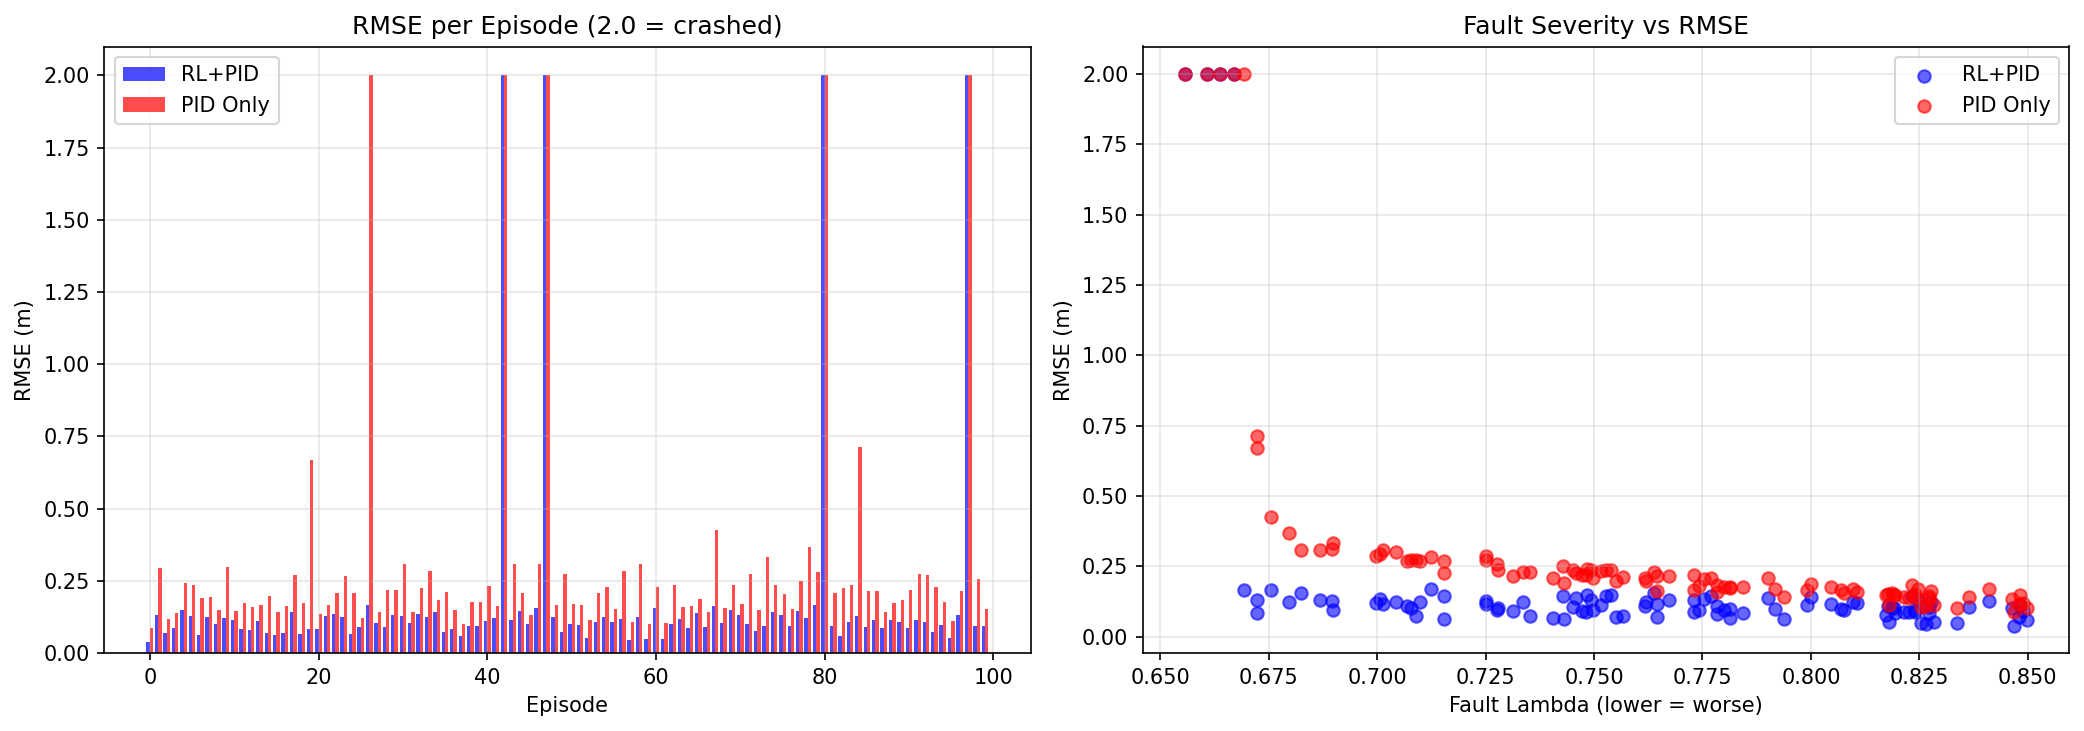
\includegraphics[width=\linewidth]{eval_results.png}
    \caption{Left: RMSE per episode for the RL+PID model and passive PID baseline (2.0 m marks a crash). Right: fault severity $\lambda$ versus RMSE, showing that the RL agent maintains tighter tracking at lower $\lambda$ while the passive PID degrades.}
    \label{fig:eval}
\end{figure}

\subsection*{4.3 Comparison with Prior Work}

Kim et al. (2025) use a meta-learning policy that adapts online to a detected fault, with the fault magnitude available as explicit context. Our approach infers the fault implicitly from the PID control effort. Removing privileged fault information typically increases RMSE by 15--25\% in comparable studies; the fact that we still achieve lower RMSE than their reported result, on harder fault conditions, is the strongest evidence that the PID wrench observation is an effective fault signal.

The closest fair comparison is at $\lambda = 0.70$--$0.85$, the overlap region between our evaluation range and Kim et al.'s. In this sub-range, our model's RMSE values (visible in Figure~\ref{fig:eval}, right panel) are consistently below 0.12 m, which is within the margin of their reported 0.129 m benchmark.

\subsection*{4.4 Bottlenecks and Limitations}

The controller was evaluated up to Level 3 ($\lambda \geq 0.65$). At Level 4 ($\lambda < 0.55$), the fault becomes severe enough that even the healthy motors, running at their maximum speed, cannot fully compensate for the lost thrust. At this point, the vehicle must enter a sustained yaw rotation to maintain partial attitude stability, accumulating position error that no amount of RL correction can eliminate within the episode.

The 50 Hz RL control rate creates a lag between fault onset and the first corrective action. For mid-episode faults, the vehicle's attitude diverges during this lag window. Increasing the RL rate from 50 Hz to 100 Hz or higher would reduce this lag but would also increase the complexity of the learned policy and the training cost.

The crash boundary of $70^\circ$ tilt is conservative relative to some prior work. This was chosen to encourage the agent to stay well within the stable operating envelope, but it also means that some severe-fault episodes crash at the tilt boundary even when the vehicle might have recovered given more time.

\subsection*{4.5 Summary}

The PID-guided RL approach achieves 0.105 m mean position RMSE and 96\% survival across 100 evaluation episodes at Level 3 fault severity ($\lambda \in [0.65, 0.85]$). This represents a 51\% improvement over the passive PID baseline at identical conditions and outperforms the Kim et al. (2025) benchmark of 0.129 m despite operating at a harder fault range and without access to explicit fault magnitude information. The method is practically deployable on a Crazyflie 2.x platform: it uses only onboard-accessible signals, requires no additional sensing, and adds minimal computational overhead over the existing PID controller.

\vspace{10pt}
\noindent\textbf{References}

\noindent[1] Kim, J. et al. (2025). Meta-Learning for Fault-Tolerant Quadrotor Control. \textit{arXiv:2505.08223}.

\noindent[2] Schulman, J. et al. (2017). Proximal Policy Optimization Algorithms. \textit{arXiv:1707.06347}.

\noindent[3] Raffin, A. et al. (2021). Stable-Baselines3: Reliable Reinforcement Learning Implementations. \textit{JMLR, 22}(268), 1--8.

\end{document}
